\section{Analisi dei Rischi}
La gestione dei rischi è un processo al quale il gruppo \Gruppo{} dà molto importanza. Questo perché incorrere in rischi potrebbe equivalere al danneggiamento del progetto, sia nella sua \glo{organizzazione} che nella sua qualità.
Si cerca quindi di fare una previsione dei problemi che si potrebbero verificare durante l'intero corso del progetto e, per ogni rischio identificato, si cerca una soluzione per poterlo evitare.

\subsection{Fasi della gestione dei rischi}
Il gruppo intende seguire i seguenti step nel processo di gestione dei rischi:
\begin{itemize}
	\item \textbf{Identificazione del rischio}: Questo è il primo step del processo e ci serve per identificare i rischi che potrebbero portare a dei problemi durante l'avanzamento del progetto; 
	\item \textbf{Analisi dei rischi}: Dopo aver individuato i rischi nello step precedente, per ognuno di essi viene valutata la probabilità che si verifichi e le conseguenze negative che potrebbe portare;
	\item \textbf{Pianificazione del rischio}: Nella pianificazione del rischio si sviluppano dei piani per sapere quali rimedi vanno intrapresi nel momento in cui i rischi si verificano. In tale maniera si riuscirà a risolvere i problemi prima che si aggravino;
	\item \textbf{Monitoraggio del rischio}: Nell'ultimo step della gestione del rischio viene verificato che le ipotesi relative ai rischi non abbiano subito delle variazioni. Quindi si cerca di valutare periodicamente la probabilità che il rischio si verifichi e i suoi possibili effetti, migliorando le strategie adottate per la loro risoluzione.
\end{itemize}

\subsection{Tipologia del rischio}
Ci sono 5 tipi di rischi che il gruppo \Gruppo{} terrà in considerazione. 
\\Ad ogni rischio verrà assegnato un codice identificativo:
\begin{itemize}
	\item Rischi Tecnologici [RT];
	\item Rischi Organizzativi [RO];
	\item Rischi Personali [RP];
	\item Rischi dei Requisiti [RR];
	\item Rischi di Stima [RS].
\end{itemize}

\subsection{Tabella dei rischi}
Nella seguente tabella vengono elencati i rischi che il gruppo \Gruppo{} potrebbe incontrare durante l'intero ciclo di vita del progetto.
Ogni riga della tabella corrisponde ad un rischio ed è composta da:
\begin{itemize}
	\item Codice [codice del tipo + numero sequenziale] e Nome del rischio;
	\item Descrizione;
	\item Rilevamento;
	\item Piano di Contingenza.
\end{itemize}

{
\rowcolors{2}{grigetto}{white}
\renewcommand{\arraystretch}{1.5}
\centering
\begin{longtable}{ c c  C{4cm}  C{3cm} C{4cm}}
\rowcolor{darkblue}
\textcolor{white}{\textbf{Codice}} & \textcolor{white}{\textbf{Nome}} & \textcolor{white}{\textbf{Descrizione}} & \textcolor{white}{\textbf{Rilevamento}} & \textcolor{white}{\textbf{Probabilità e Gravità}} & \textcolor{white}{\textbf{Risoluzione}}\\	

RT1 & Inesperienza alle tecnologie & Il gruppo dovrà affrontare tecnologie mai utilizzate precedentemente e quindi servirà del tempo per poter imparare ad utilizzarle nel modo corretto & Ogni componente del gruppo sarà consapevole di saper usare una determinata tecnologia & Probabilità Alta Gravità Media & Ogni componente del gruppo che ha acquisito una certa abilità nell'utilizzo di una tecnologia, cercherà di aiutare i componenti del gruppo che hanno più difficoltà \\
		

\end{longtable}
}

\subsection{Occorrenza delle situazioni di rischio}
In questa sezione viene descritto quanto i rischi indicati in §2.3 si sono effettivamente verificati durante lo svolgimento del progetto.
\subsubsection{Fase di Analisi}
{
\rowcolors{2}{grigetto}{white}
\renewcommand{\arraystretch}{2}
\centering
\begin{longtable}{C{2cm} C{3cm} C{10cm}}
\caption{Tabella occorrenza e mitigazione nella Fase di Analisi}\\
\rowcolor{darkblue}

\textcolor{white}{\textbf{Codice}} & 
\textcolor{white}{\textbf{Occorrenza}} & 
\textcolor{white}{\textbf{Descrizione e risoluzione}}\\	
\endhead

RT1 &
Bassa &
Tutti i membri del gruppo hanno dovuto apprendere il linguaggio \LaTeX{} inoltre Christian e Riccardo l'utilizzo di \glo{Git}, in quanto mai usato prima. Entrambi non hanno portato gravi ripercussioni sull'avanzamento del progetto in quanto rapidamente apprendibili (per i nostri scopi). \\

RP1 &
Bassa &
Le decisioni prese sono state generalmente accolte positivamente da tutti i membri del gruppo. Nella definizione degli attori e dei requisiti ci sono state maggiori difficoltà ad accordarsi, poi risolte durante l'incontro con il proponente. In generale, le maggiori difficoltà sono state comunque dovute all'incomprensione, poi risolte con la redazione del \Glossario. \\

RP2 &
Bassa &
Non ci sono stati particolari problemi di comunicazione con il proponente. È stato richiesto un incontro per poter discutere di dubbi che si sono presentati durante l'analisi ed è stato proficuo. \\

RR1 &
Media &
Come indicato in RP1, c'è stata disattenzione nella definizione di alcuni requisiti sfociata in difficoltà di comprensione fra i membri del gruppo. Dopo l'incontro con il proponente, queste situazioni di incomprensione sono state risolte. \\

RS1 &
Alta &
Considerando il poco tempo a disposizione e gli impegni di ogni membro del gruppo sono state richieste più ore di quante preventivate per lo svolgimento delle attività. Complice di questo errore è anche non aver preventivato in maniera ottimale la suddivisione dei tempi. Sono stati quindi suddivisi nuovamente i compiti e cercato di collaborare e comunicare il più possibile in remoto, al fine di raggiungere gli obiettivi prestabiliti. \\

RO1 &
Media &
Pur di rispettare le \glo{milestone} ogni membro del gruppo ha cercato di supportarsi a vicenda nel tentativo di rispettare le scadenze, purtroppo non sempre con successo. \\

RO2 &
Media &
Per mancata esperienza l'assegnazione di alcune scadenze sono risultate sbagliate o pianificate male. Alla luce degli errori commessi, deve essere effettuata una miglior pianificazione delle attività. \\

RO3 &
Alta &
È stato organizzato un solo incontro con il proponente che, seppur proficuo, non è sufficiente per accertarsi di essere in sintonia con esso. Nei prossimi periodi deve esserci una maggior comunicazione, anche attraverso l'utilizzo di \glo{Slack} per una maggiore interazione. \\

RO4 &
Bassa &
Essendo ancora periodo di lezioni, non ci sono stati problemi nell'incontrarci, anche perché gli incontri sono sempre stati fissati con almeno una settimana di anticipo. \\

\end{longtable}	
}

\subsubsection{Fase di Progettazione Architetturale}
{
\rowcolors{2}{grigetto}{white}
\renewcommand{\arraystretch}{2}
\centering
\begin{longtable}{C{2cm} C{3cm} C{10cm}}
\caption{Tabella occorrenza e mitigazione nella Fase di Progettazione Architetturale}\\
\rowcolor{darkblue}

\textcolor{white}{\textbf{Codice}} & 
\textcolor{white}{\textbf{Occorrenza}} & 
\textcolor{white}{\textbf{Descrizione e risoluzione}}\\	
\endhead

RT1 &
Alta &
Tutti i membri del gruppo hanno dovuto apprendere dei linguaggi e strumenti in base al compito che gli è stato assegnato. I linguaggi/strumenti presi in causa sono i seguenti: \glo{CSS}, \glo{HTML5}, \glo{JSON}, \glo{TypeScript}, \glo{Node.js}, \glo{MySQL}, \glo{Redis}, \glo{YAML}, \glo{Swagger}, \glo{OpenAPI}, \glo{Spring}, \glo{Maven}, \glo{Java} e Android Studio. Il tempo per apprendere queste tecnologie in maniera sufficiente è stato abbastanza dispendioso. In alcuni casi lo studio ha occupato più tempo del previsto ma in conclusione siamo riuscito a realizzare il \glo{PoC} funzionante. \\

RP1 &
Bassa &
Le decisioni prese sono state generalmente accolte positivamente da tutti i membri del gruppo. C'è stata qualche difficoltà sulla scelta per la realizzazione dei collegamenti tra le varie parti del \glo{PoC} (app, web-app e server) e farli funzionare correttamente; anche per l'utilizzo di certe tecnologie, varie compatibilità e versioni. In generale dopo una discussione tra i vari membri del gruppo si riusciva a venirsi incontro con le decisioni. \\

RP2 &
Bassa &
Non ci sono stati particolari problemi di comunicazione con il proponente. È stato richiesto un incontro in videoconferenza per discutere di alcuni dubbi che si sono presentati durante la scelta di certe tecnologie, linguaggi, versioni e librerie che ha aiutato alla realizzazione del \glo{PoC}. \\

RR1 &
Bassa &
Ci sono stati dubbi su alcuni requisiti e casi d'uso presentati nell'\AdRv{2.0.0}. È stata svolta una videochiamata sulla piattaforma \glo{Hangouts} con \CR{} per risolvere dubbi ed incomprensioni. \\

RS1 &
Bassa &
Per quanto riguarda lo studio delle tecnologie, la realizzazione del \glo{PoC} e la correzione dei documenti quasi tutti i tempi richiesti sono stati rispettati (in particolar modo rispetto alla precedente fase in cui l'occorrenza era stata alta). \\

RO1 &
Bassa &
Pur di rispettare le \glo{milestone} ogni membro del gruppo ha cercato di supportarsi a vicenda nel tentativo di rispettare le scadenze. In particolar modo, nonostante la suddivisione del lavoro in tre parti (e quindi gruppi di membri) ci si è comunque aiutati pur di completare il lavoro. \\

RO2 &
Bassa &
Avendo acquisito maggior esperienza nell'assegnazione di alcune scadenze sono state quasi tutte rispettate e non è servita uno stravolgimento della pianificazione. Alla luce degli errori commessi nel RR, la pianificazione ha ottenuto maggiore importanza. \\

RO3 &
Media &
È stato organizzato un solo incontro con il proponente che è stato molto proficuo. Alcuni dubbi si sono risolti attraverso l'utilizzo di \glo{Slack} per una maggiore interazione. \\

RO4 &
Media &
Essendo la fase cominciata nel periodo esami, ogni membro del gruppo aveva altri impegni importanti da rispettare.
In aggiunta ad essi, alla fine della sessione si è verificata un'altra situazione che ha complicato l'avanzamento dei lavori, ovvero la diffusione del Covid-19 che ha portato disagi come la chiusura delle aule universitarie, limitazioni di trasporti e di comunicazioni.
Il lavoro è stato necessariamente compiuto sfruttando al massimo le potenzialità che gli strumenti \glo{Discord}, \glo{Slack} e \glo{Hangouts} offrono.
L'organizzazione avveniva su \glo{Slack} mentre su \glo{Discord} avvenivano le chiamate vocali e le condivisioni degli schermi dei computer in live streaming.
I colloqui con committente e proponente sono dovuti avvenire attraverso \glo{Hangouts}, con la importante limitazione del numero di utenti in una chiamata (fisso a 6). \\

\end{longtable}	
}

\subsubsection{Fase di Progettazione di Dettaglio e Codifica}
{
\rowcolors{2}{grigetto}{white}
\renewcommand{\arraystretch}{2}
\centering
\begin{longtable}{C{2cm} C{3cm} C{10cm}}
\caption{Tabella occorrenza e mitigazione nella Fase di Progettazione di Dettaglio e Codifica}\\
\rowcolor{darkblue}

\textcolor{white}{\textbf{Codice}} & 
\textcolor{white}{\textbf{Occorrenza}} & 
\textcolor{white}{\textbf{Descrizione e risoluzione}}\\	
\endhead

RT1 &
Alta &
Nonostante gran parte del lavoro di apprendimento delle tecnologie fosse già stato fatto per la realizzazione del \glo{PoC}, al fine di ottenere un prodotto software più mantenibile è stato necessario occupare altro tempo per riuscire ad ottenere un livello di dettaglio maggiore. Questo non ha purtroppo dato vantaggi dal punto di vista del rispetto dei tempi, certamente però ha migliorato la qualità del prodotto e la comprensione delle tecnologie. Nella prossima e ultima fase è necessario che le tecnologie da usare siano consolidate per evitare che il problema si ripresenti, così facendo si riuscirebbe a evitare questo rischio. \\

RP1 &
Media &
Il metodo fin qui adottato di discussione fra le componenti del gruppo in disaccordo, discutendo sui pro e contro di ogni proposta, si è rivelato efficace. Per valutare pro e contro si sono sempre confrontate le proposte con le best practice di dominio (riguardanti le architetture e le tecnologie coinvolte). \\

RP2 &
Bassa &
In caso il proponente non risponda alle e-mail, è possibile contattarlo tramite un canale \glo{Telegram} che ci è stato messo a disposizione per comunicare in maniera più diretta. Essendo questo canale utilizzabile da tutti i gruppi che stanno svolgendo il progetto \NomeProgetto{}, è bene non abusarne. \\

RR1 &
Bassa &
I requisiti raccolti sono risultati sufficienti a portare avanti lo sviluppo del progetto. I problemi evidenziati dal committente al documento \AdR{} sono stati risolti senza particolari problemi, anche grazie alle ultime lezioni di esercitazione del corso di Ingegneria del Software. \\

RS1 &
Alta &
Conseguenza diretta di RT1 e RO1. \\

RO1 &
Alta &
Alla luce di quanto indicato in RT1, e in vista dell'imminente esame del corso di Ingegneria del Software è stato deciso, per evitare di risultare inconcludenti, di posticipare le scadenze. I periodi della fase corrente sono stati raggruppati a quelli della fase successiva. La scelta è stata corretta, soprattutto a posteriori. Alla fine del periodo 1 dell'ultima fase del progetto è bene esplorare nuovamente questa ipotesi, se dovesse essere necessario (l'auspicio è che non serva). \\

RO2 &
Media &
Con le nuove scadenze fissate, come indicato, in RO1 il rispetto delle \glo{milestone} è stato fatto con più agevolezza. \\

RO3 &
Bassa &
A questo stadio di sviluppo la comunicazione con il proponente è stata ridotta al solo necessario per alcuni dettagli implementativi, per le parti al gruppo poco chiare. Queste modalità fino ad ora adottate si sono rivelate valide. \\

RO4 &
Bassa &
Non ci sono stati problemi di comunicazione in quanto è avvenuta solamente tramite i canali di comunicazione così come indicate nelle \NdP{}: \glo{Discord} e \glo{Slack}. \\

\end{longtable}	
}
\newpage

\subsubsection{Fase di Validazione e Collaudo}
{
\rowcolors{2}{grigetto}{white}
\renewcommand{\arraystretch}{2}
\centering
\begin{longtable}{C{2cm} C{3cm} C{10cm}}
\caption{Tabella occorrenza e mitigazione nella Fase di Validazione e Collaudo}\\
\rowcolor{darkblue}

\textcolor{white}{\textbf{Codice}} & 
\textcolor{white}{\textbf{Occorrenza}} & 
\textcolor{white}{\textbf{Descrizione e risoluzione}}\\	
\endhead

RT1 &
Bassa &
Il gruppo al termine di questo progetto può sentirsi in grado di padroneggiare le tecnologie utilizzate nel modo sufficiente a poterlo portare a termine. Il consolidamento della propria conoscenza nell'uso di queste tecnologie è quindi riuscito e quindi un loro uso futuro in altri ambiti lavorativi sarà certamente più agevole. \\

RP1 &
Bassa &
Non ci sono stati conflitti decisionali, in quanto le scelte da effettuare sono state su temi non così importanti da poter accendere discussioni. Ad ogni modo, il metodo fin qui adottato si è rivelato valido e può essere quindi sfruttato come conoscenza e farlo diventare parte del personale \glo{way of working}. \\

RP2 &
Bassa &
Il proponente ha sempre risposto celermente alle comunicazioni via e-mail, di conseguenza si è scelto di utilizzarlo nuovamente come metodo principale di comunicazione. La quantità di volte con cui si è entrati in contatto è stata corretta (all'inizio e alla fine di questa fase) ed è stata sufficiente per poter portare a termine il progetto. \\

RR1 &
Bassa &
I requisiti raccolti sono risultati sufficienti a portare avanti lo sviluppo del progetto. I problemi evidenziati dal committente al documento \AdR{} sono stati risolti senza particolari problemi, anche grazie alla comunicazione via e-mail avuta con egli. \\

RS1 &
Bassa &
Le milestone sono state correttamente rispettate, grazie anche al fatto che il lavoro rimasto era comunque inferiore a quanto avuto fino alla scorsa valutazione delle occorrenze dei rischi. \\

RO1 &
Bassa &
Come per RS1. \\

RO2 &
Bassa &
Dovuto a RS1, il calendario delle scadenze è stato rispettato con correttezza e quindi la nuova pianificazione è stata correttamente realizzata. \\

RO3 &
Bassa &
Come indicato in RP2, non si sono presentati problemi nella comunicazione con il proponente. \\

RO4 &
Bassa &
Non ci sono stati problemi di comunicazione in quanto è avvenuta solamente tramite i canali di comunicazione così come indicate nelle \NdP{}: \glo{Discord} e \glo{Slack}. \\

\end{longtable}	
}

\subsubsection{Andamento dell'occorrenza dei rischi}

\pgfplotsset{width=17cm, height=6cm}
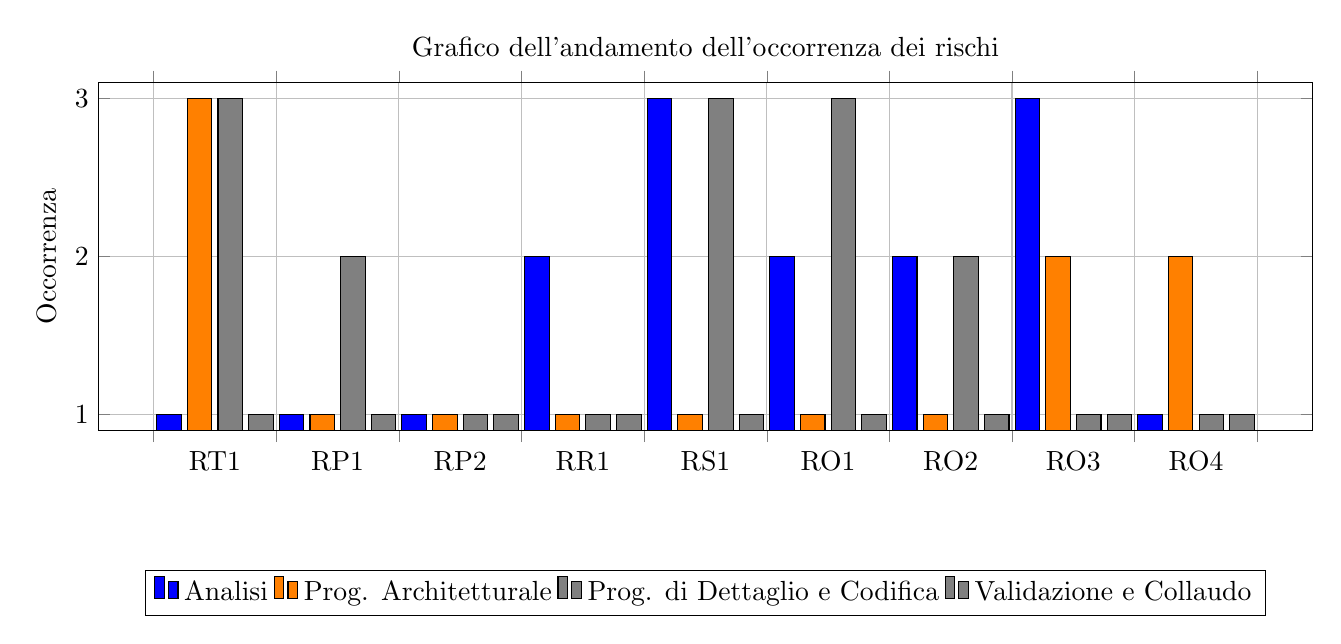
\begin{tikzpicture}

\begin{axis}[
title=Grafico dell'andamento dell'occorrenza dei rischi,
x tick label style={
	/pgf/number format/1000 sep=},
ylabel=Occorrenza,
enlargelimits=0.05,
legend style={at={(0.5,-0.4)},
	anchor=north,legend columns=-1},
ybar interval=0.8,
ytick={1,2,3},
symbolic x coords={RT1, RP1, RP2, RR1, RS1, RO1,
	RO2, RO3, RO4, tmp},%lasciare tmp come ultima colonna per poter visualizzare tutte le colonne tranne tmp
% x tick label style={rotate=45,anchor=east},
grid=major,
xtick=data
]
\addplot[fill=blue] coordinates {
	(RT1, 1) (RP1, 1) (RP2, 1) 
	(RR1, 2) (RS1, 3) (RO1, 2)
	(RO2, 2) (RO3, 3) (RO4, 1) (tmp, 3)
};

\addplot [fill=orange] coordinates {
	(RT1, 3) (RP1, 1) (RP2, 1) 
	(RR1, 1) (RS1, 1) (RO1, 1)
	(RO2, 1) (RO3, 2) (RO4, 2) (tmp, 3)
};

\addplot [fill=gray] coordinates {
	(RT1, 3) (RP1, 2) (RP2, 1) 
	(RR1, 1) (RS1, 3) (RO1, 3)
	(RO2, 2) (RO3, 1) (RO4, 1) (tmp, 3)
};

\addplot [fill=gray] coordinates {
	(RT1, 1) (RP1, 1) (RP2, 1) 
	(RR1, 1) (RS1, 1) (RO1, 1)
	(RO2, 1) (RO3, 1) (RO4, 1) (tmp, 3)
};

\legend{
	Analisi,
	Prog. Architetturale,
	Prog. di Dettaglio e Codifica,
	Validazione e Collaudo
}
\end{axis}
\end{tikzpicture}

\mbox{}\\
Il grafico qui riportato rappresenta l'andamento del verificarsi dell'occorrenza dei rischi e permette di analizzare quanto un rischio abbia rispettato o meno il suo livello di gravità durante una fase.
Grazie a questo grafico è possibile comprendere che i rischi più frequenti sono quelli di tipo organizzativi, che però nell'avanzare del progetto, in media, migliorano.
Si può notare, invece, di aver sottostimato i rischi tecnologici, la cui gravità da media viene portata a livello alto.